\section{Introduction}
\label{sec:introduction}

\subsection{Overview of High-Frequency Trading and Reinforcement Learning}
High-frequency trading represents one of the most technologically demanding domains within quantitative finance,
characterized by a need for ultra-low latency, massive volumes of data streaming, and the ability to dynamically adapt to changing market conditions.
Reinforcement learning has emerged as a promising approach for developing trading strategies within the context of high-frequency trading (HFT),
offering the ability to learn optimal policies directly from market interactions without requiring explicit knowledge of the underlying dynamics.
However, existing reinforcement learning algorithms are fraught with challenges,
particularly regarding scaling training and inference to meet the performance requirements of live trading environments.

Traditional frameworks often rely on centralized architectures, where a single learner aggregates experiences from multiple actors to update a shared policy.
While effective in general-purpose applications, such approaches can become bottlenecks in HFT contexts,
where the scale and complexity of trading environments demand highly efficient distributed training.
Moreover, typical RL systems treat environments as isolated entities for each agent or strategy,
leading to significant computational redundancies when simulating complex environments with shared attributes, like a limit order book (LOB).
The LOB is a critical component in the high-frequency trading ecosystem, representing the collection of all outstanding buy and sell orders in a market,
and are crucial for understanding the dynamics of price formation and liquidity provision.

\subsection{Limit Order Book Environments}
A LOB is typically represented as a list of price levels, each containing the aggregated volume of orders at that price.
For example, in a simplified book with four price levels, the bid side (buy orders) and ask side (sell orders) might look as follows:

\begin{table}[H]
    \centering
    \makebox[\textwidth]{
        \begin{minipage}{0.45\textwidth}
            \raggedleft
            \begin{tabular}{|c|c|}
                \hline
                \textbf{Price Level} & \textbf{Volume} \\ \hline
                101.71               & 31              \\ \hline
                101.84               & 56              \\ \hline
                101.95               & 42              \\ \hline
                102.01               & 9               \\ \hline
            \end{tabular}
        \end{minipage}
        \hspace{0.5cm}
        \begin{minipage}{0.45\textwidth}
            \begin{tabular}{|c|c|}
                \hline
                \textbf{Price Level} & \textbf{Volume} \\ \hline
                102.64               & 44              \\ \hline
                102.66               & 31              \\ \hline
                102.72               & 26              \\ \hline
                102.85               & 13              \\ \hline
            \end{tabular}
        \end{minipage}
    }
    \caption{Bid (left) and Ask (right) sides of a Limit Order Book (LOB) $L$}
    \label{tab:lob}
\end{table}

In this example, the bid side contains four price levels with corresponding volumes of 31, 56, 42, and 9, respectively,
while the ask side contains four price levels with volumes of 44, 31, 26, and 13.
The difference between the best bid and ask prices is known as the bid-ask spread, which in this case is $\Delta = 102.01 - 102.64 = -0.63$.
A visualization of the LOB accumulated depth for this example is shown in~\hyperref[fig:lob]{Figure~\ref{fig:lob}}.

\begin{figure}[H]
    \centering
    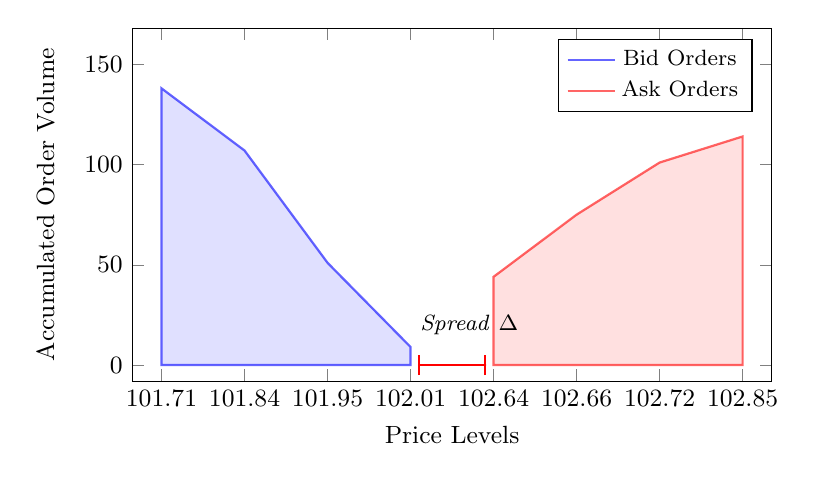
\begin{tikzpicture}
        \begin{axis}[
            ymin=0, ymax=160,
            xlabel={Price Levels},
            ylabel={Accumulated Order Volume},
            width=0.8\textwidth, height=0.5\textwidth, % Reduce figure size
            xticklabels={101.71, 101.84, 101.95, 102.01, 102.64, 102.66, 102.72, 102.85},
            xtick={1,2,3,4,5,6,7,8},
            enlargelimits=0.05,
            legend pos=north east, % Adjust legend position
            legend style={font=\footnotesize}, % Make legend smaller
            ylabel style={yshift=4pt}, % Slight adjustment for label
            font=\small % Reduce overall font size
        ]

            % Bid Curve (Cumulative)
            \addplot [blue, thick, fill=blue!20, opacity=0.6] coordinates {
                (1, 138) (2, 107) (3, 51) (4, 9)
            } \closedcycle;
            \addlegendentry{Bid Orders}

            % Ask Curve (Cumulative)
            \addplot [red, thick, fill=red!20, opacity=0.6] coordinates {
                (5, 44) (6, 75) (7, 101) (8, 114)
            } \closedcycle;
            \addlegendentry{Ask Orders}

            % Bid-Ask Spread Indicator
            \draw [red, thick, line cap=round] (axis cs:4.1,0) -- (axis cs:4.9,0);
            \draw [red, thick] (axis cs:4.1,-5) -- (axis cs:4.1,5);
            \draw [red, thick] (axis cs:4.9,-5) -- (axis cs:4.9,5);
            \node[right, font=\footnotesize] at (axis cs:4,20) {\textit{Spread} $\Delta$};

        \end{axis}
    \end{tikzpicture}
    \caption{Limit Order Book Depth visualization for an arbitrary LOB $L$}
    \label{fig:lob}
\end{figure}

\subsection{Motivation and Contributions}

The main contribution of this course conclusion thesis is the design and comparison of a parallel agent-based RL framework for HFT applications.
We aim to leverage the Ray RLLib framework to parallelize environments and use ZeroMQ for brokerless communication between workers and environments,
inspired by the actor-learner model introduced in the IMPALA (Importance Weighted Actor-Learner Architecture) algorithm.
However, we extend the original implementation by allowing multiple learners to share multiple environments,
enabling unique learners to interact with the same LOB environment, as shown in~\hyperref[fig:framework]{Figure~\ref{fig:framework}}.

The reduced computational overhead by reusing core environment components, such as order aggregation, order book initialization,
and transaction processing, across multiple agents, could lead to significant performance improvements in terms of speedup and multicore efficiency.
We will measure wall time latency from environment step to agent action output as the primary metric for evaluating the framework's performance,
and change in agent loss and reward scores as secondary metrics for assessing the framework's sensibility to multi-agent environments.
The primary contribution of the thesis is to provide a scalable
and adaptable framework for training RL agents in HFT applications, with the following key features:

\begin{itemize}
    \item A parallel agent-based framework: A system architecture to enable efficient and decoupled training of multiple RL agents
    by leveraging distributed computing resources.

    \item Shared limit order book environments: A mechanism for reducing redundant computations by allowing multiple workers
    to interact with shared reusable environment.

    \item Continuous train-and-deploy pipeline: Support dynamic training and deployment of multiple strategies,
    where learners can be added or removed without disrupting the training process.
\end{itemize}

The framework must scale effectively with the number of agents, learners, and environments, maintaining consistent performance as workload increases.
Performance metrics will include speedup and multicore efficiency, processing latency per action and end-to-end latency from state observation to order sending.
The framework will be evaluated for its ability to support diverse trading strategies
and market conditions through strategy-agnostic performance and modular design,
enabling the reconfiguration of agent definitions and environments with minimal overhead.
Additionally, the strategies will be evaluated based on simulated loss and reward scores and the sensibility to multiple agent interactions.

The final thesis structure will first review relevant literature and novel approaches towards distributed agents
in reinforcement learning and intersections with high-frequency trading, specifically parallel environments.
An adequate search string will be fabricated, and a systematic review will be conducted to identify the most relevant literature,
with a final discussion on the tagged literature and the relevance of each foundational paper to the proposed framework.
Further discussion into the problem formulation and system design, providing a description of the proposed state, action and reward spaces will be made.
The implementation of the framework will then be discussed, covering technical aspects and the integration of the various computational components,
such as how the message passing between workers and learners will be made, and how the policy networks interaction with simulation dynamics are handled.
Experimental results will be presented to evaluate the performance and scalability of the framework, both in the computational and financial domains.
Finally, the thesis will conclude with a summary of results and a discussion of potential future directions for further research and developments.

\begin{figure}[H]
    \centering
    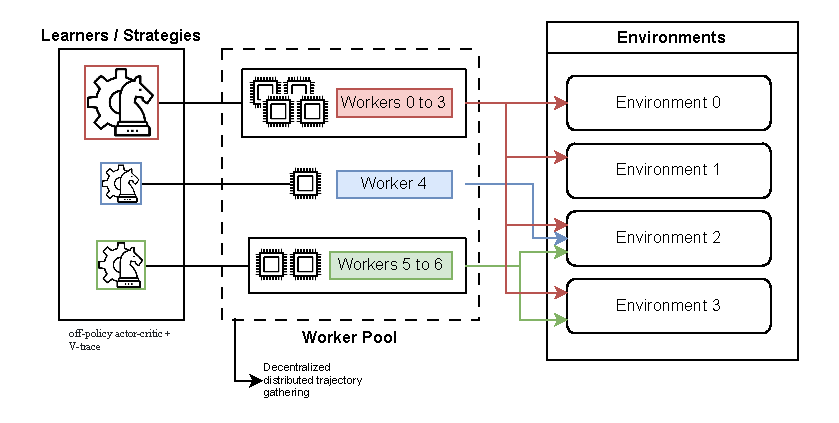
\includegraphics[width=\textwidth]{diagram}
    \caption{Diagram for the proposed parallel agent-based framework, with worker-learner interactions and shared limit order book environments.}
    \label{fig:framework}
\end{figure}

